\begin{figure}[htbp]
    \centering
    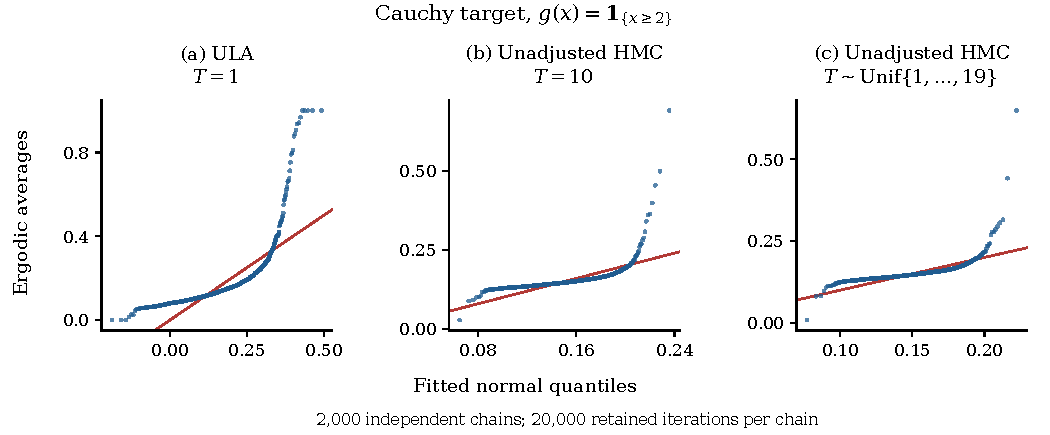
\includegraphics[width=\textwidth]{figures/01_ula_fixed_random.pdf}
    \caption{Gaussian QQ plots of first absolute-moment averages for ULA,
    unadjusted HMC with $T=10$ leapfrog steps, and unadjusted HMC with an
    independent $T\sim\mathrm{Unif}\{1,\ldots,19\}$ at each iteration.
    The potential is $U(x)=2\log(1+x^2/3)$, corresponding to the Student
    $t$ distribution with three degrees of freedom, and $g(x)=|x|$.
    This observable has a finite second moment under the target law.
    Each panel contains 2,000 independent chains started at zero, run for
    120,000 iterations with the first 40,000 discarded; each point is an
    average over the remaining 80,000 observations. Step size is $h=0.35$,
    mass is one, and tuning is fixed.
    Vertical coordinates are the ordered raw chain averages; horizontal
    coordinates are Gaussian quantiles fitted using their sample mean and
    standard deviation. There is no $\sqrt n$ scaling. The line is $y=x$;
    axis limits are chosen separately and every average is shown.
    All three kernels are unadjusted and may have invariant-distribution
    bias. These finite-run plots illustrate distributional shape rather
    than establish a CLT or its failure.}
    \label{fig:ula-fixed-random}
\end{figure}
